\documentclass[aspectratio=169,10pt]{beamer}

%──────────────────────────────────────────────────────────────────
%  Theme & colours
%──────────────────────────────────────────────────────────────────
\usetheme{metropolis}
\metroset{sectionpage=none,subsectionpage=none}
\usepackage{appendixnumberbeamer}

\definecolor{DarkBlue}{HTML}{1a1a2e}
\definecolor{MidBlue}{HTML}{16213e}
\definecolor{AccentBlue}{HTML}{0f3460}
\definecolor{AccentPurple}{HTML}{533483}
\definecolor{NeonPink}{HTML}{e94560}
\definecolor{AccentText}{HTML}{FFB8CC}
\definecolor{SoftWhite}{HTML}{f0f0f0}
\definecolor{LightGray}{HTML}{d0d0d0}
\definecolor{Black}{HTML}{000000}

\setbeamercolor{background canvas}{bg=DarkBlue}
\setbeamercolor{normal text}{fg=SoftWhite}
\setbeamercolor{frametitle}{bg=MidBlue,fg=SoftWhite}
\setbeamercolor{title separator}{fg=AccentText}
\setbeamercolor{progress bar}{fg=AccentText,bg=AccentBlue}
\setbeamercolor{block title}{bg=AccentPurple,fg=SoftWhite}
% \setbeamercolor{block body}{bg=AccentBlue!60,fg=SoftWhite}
\setbeamercolor{block body}{bg=Black!80,fg=SoftWhite}
\setbeamercolor{alerted text}{fg=AccentText}
\setbeamercolor{itemize item}{fg=AccentText}
\setbeamercolor{itemize subitem}{fg=LightGray}
\setbeamercolor{section in toc}{fg=SoftWhite}

%──────────────────────────────────────────────────────────────────
%  Packages
%──────────────────────────────────────────────────────────────────
\usepackage{tikz}
\usetikzlibrary{arrows.meta,positioning,decorations.pathreplacing,
                shapes.geometric,backgrounds,calc,fit,fadings}
\usepackage{amsmath,amssymb,bm}
\usepackage{booktabs}
% fontawesome5 not available; using text icons
\newcommand{\faIcon}[1]{\textbullet}
\usepackage{pgfplots}
\pgfplotsset{compat=1.18}
\usepackage{xcolor}
\usepackage{mathtools}

%──────────────────────────────────────────────────────────────────
%  Metadata
%──────────────────────────────────────────────────────────────────
\title{\textbf{Diffusion Models}}
\subtitle{How AI Learns to Create Images from Noise}
\author{Presented by: \textit{Anindya, Tamal and Din}}
\date{\today}
\institute{Course Presentation}

%──────────────────────────────────────────────────────────────────
%  Custom commands
%──────────────────────────────────────────────────────────────────
\newcommand{\x}{\mathbf{x}}
\newcommand{\eps}{\boldsymbol{\varepsilon}}
\newcommand{\highlight}[1]{\textcolor{AccentText}{\textbf{#1}}}
\newcommand{\soft}[1]{\textcolor{LightGray}{#1}}

% ─── Noise-level boxes ───────────────────────────────────────────
\newcommand{\noisebox}[2]{%
  \begin{tikzpicture}[baseline=-2pt]
    \node[rounded corners=3pt,fill=#1,minimum width=1.1cm,
          minimum height=0.6cm,font=\tiny\bfseries,text=white]{#2};
  \end{tikzpicture}}

%══════════════════════════════════════════════════════════════════
\begin{document}
%══════════════════════════════════════════════════════════════════

%──────────────────────────────────────────────────────────────────
% TITLE SLIDE
%──────────────────────────────────────────────────────────────────
{
\setbeamercolor{background canvas}{bg=DarkBlue}
\begin{frame}[plain]
  \begin{tikzpicture}[remember picture,overlay]
    % decorative circles
    \foreach \r/\op in {5/0.05,3.5/0.08,2/0.12}{
      \fill[NeonPink,opacity=\op]
        (current page.north east) circle (\r cm);
    }
    \foreach \r/\op in {4/0.05,2.5/0.08,1.2/0.12}{
      \fill[AccentPurple,opacity=\op]
        (current page.south west) circle (\r cm);
    }
  \end{tikzpicture}
  \vspace{1.4cm}
  \titlepage
\end{frame}
}

%──────────────────────────────────────────────────────────────────
% OUTLINE
%──────────────────────────────────────────────────────────────────
\begin{frame}{Roadmap}
  \vspace{0.3cm}
  \begin{columns}[T]
    \column{0.55\textwidth}
      \tableofcontents
    \column{0.42\textwidth}
      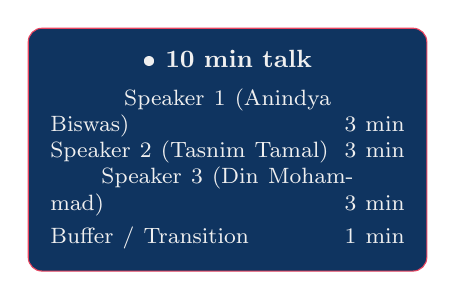
\begin{tikzpicture}
        \node[draw=NeonPink,rounded corners=5pt,
              text=SoftWhite,fill=AccentBlue,
              text width=4.5cm, align=center, inner sep=8pt]{
          \small
          \faIcon{clock}~\textbf{10 min talk}\\[4pt]
          \footnotesize
          Speaker 1 (Anindya Biswas) \hfill 3 min\\
          Speaker 2 (Tasnim Tamal) \hfill 3 min\\
          Speaker 3 (Din Mohammad) \hfill 3 min\\
          Buffer / Transition \hfill 1 min
        };
      \end{tikzpicture}
  \end{columns}
\end{frame}

%══════════════════════════════════════════════════════════════════
\section{Motivation}
%══════════════════════════════════════════════════════════════════

\begin{frame}{Why Diffusion Models?}
  \begin{columns}[T]
    \column{0.54\textwidth}
      \begin{block}{In One Line}
        A diffusion model learns to \highlight{turn random noise into meaningful data}
        (like realistic images).
      \end{block}
      \vspace{6pt}
      \begin{itemize}
        \item \textbf{GANs}: high quality, but training is often unstable
        \item \textbf{VAEs}: stable and fast, but outputs can look blurry
        \item \textbf{Flows}: mathematically clean, but architecture is restricted
        \item \highlight{Diffusion}: stable training + very strong output quality
      \end{itemize}
      \vspace{6pt}
      \soft{Used in tools like DALL·E 3, Stable Diffusion, and Sora}

    \column{0.44\textwidth}
      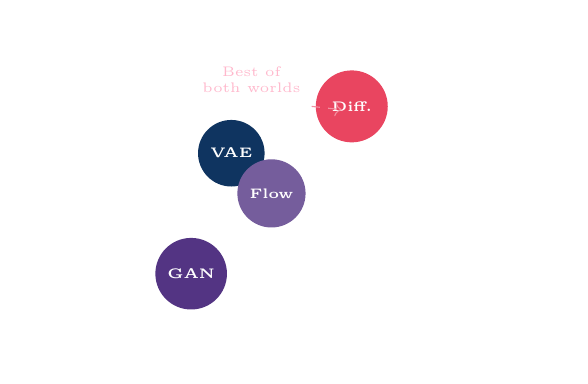
\begin{tikzpicture}[scale=0.85]
        % axes
        \draw[->,thick,white] (0,0) -- (4.5,0)
              node[right,font=\tiny]{Sample Quality};
        \draw[->,thick,white] (0,0) -- (0,4.2)
              node[above,font=\tiny]{Training Stability};
        % methods
        \node[circle,fill=AccentPurple,minimum size=22pt,
              font=\tiny\bfseries,text=white]
              at (1.2,1.0) {GAN};
        \node[circle,fill=AccentBlue,minimum size=22pt,
              font=\tiny\bfseries,text=white]
              at (1.8,2.8) {VAE};
        \node[circle,fill=AccentPurple!80,minimum size=22pt,
              font=\tiny\bfseries,text=white]
              at (2.4,2.2) {Flow};
        \node[circle,fill=NeonPink,minimum size=26pt,
              font=\tiny\bfseries,text=white]
              at (3.6,3.5) {Diff.};
        % annotation
        \draw[dashed,NeonPink!60,->] (3.0,3.5) -- (3.45,3.45);
          \node[AccentText,font=\tiny,align=center] at (2.1,3.9)
              {Best of\\ both worlds};
      \end{tikzpicture}
  \end{columns}
\end{frame}

%══════════════════════════════════════════════════════════════════
\section{Forward Process}
%══════════════════════════════════════════════════════════════════

\begin{frame}{The Forward (Noising) Process}

  \begin{block}{Key Idea}
    Gradually corrupt data $\x_0$ into pure Gaussian noise $\x_T$
    through a fixed Markov chain.
  \end{block}

  \vspace{6pt}
  \begin{equation*}
    q(\x_t \mid \x_{t-1}) = \mathcal{N}\!\left(\x_t;\;
      \sqrt{1-\beta_t}\,\x_{t-1},\;\beta_t \mathbf{I}\right)
  \end{equation*}

  \vspace{4pt}
  \begin{center}
  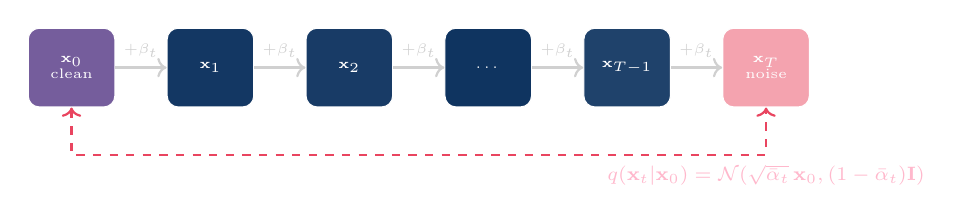
\begin{tikzpicture}[node distance=0.6cm and 0.65cm,
    box/.style={rounded corners=4pt,draw=white!40,
                fill=AccentBlue,minimum height=1.0cm,
                minimum width=1.1cm,font=\tiny,text=white,
                inner sep=2pt,align=center}]

    \node[box,fill=AccentPurple!80] (x0) {$\x_0$\\\tiny clean};
    \node[box] (x1) [right=of x0]   {$\x_1$};
    \node[box] (x2) [right=of x1]   {$\x_2$};
    \node[box] (xd) [right=of x2]   {\ldots};
    \node[box] (xt) [right=of xd]   {$\x_{T-1}$};
    \node[box,fill=NeonPink!50] (xT) [right=of xt] {$\x_T$\\\tiny noise};

    \foreach \a/\b in {x0/x1,x1/x2,x2/xd,xd/xt,xt/xT}{
      \draw[->,thick,LightGray] (\a) -- (\b)
            node[midway,above,font=\tiny]{$+\beta_t$};
    }

    % noise icons (fuzzy fills)
    \foreach \n/\op in {x1/20,x2/40,xt/70,xT/100}{
      \fill[white,opacity=0.0\op,rounded corners=4pt]
        (\n.south west) rectangle (\n.north east);
    }

    % closed-form shortcut
    \draw[<->,dashed,NeonPink,thick]
      (x0.south) -- ++(0,-0.6) -| (xT.south)
      node[midway,below,font=\scriptsize,text=AccentText]{
        $q(\x_t|\x_0)=\mathcal{N}(\sqrt{\bar\alpha_t}\,\x_0,
        (1-\bar\alpha_t)\mathbf{I})$};
  \end{tikzpicture}
  \end{center}

  \vspace{4pt}
  \small
  Plainly: start from a real sample and add a little noise repeatedly
  until almost all information is gone.

\end{frame}

%══════════════════════════════════════════════════════════════════
\section{Reverse Process}
%══════════════════════════════════════════════════════════════════

\begin{frame}{The Reverse (Denoising) Process}

  \begin{columns}[T]
    \column{0.54\textwidth}
      \textbf{Goal}: Learn $p_\theta(\x_{t-1}|\x_t)$ to reverse the noise.

      \vspace{6pt}
      A \highlight{neural network} $\eps_\theta$ predicts the noise
      present at each step:
      \begin{equation*}
        \x_{t-1} \approx \x_t - \text{predicted noise}
      \end{equation*}

      \vspace{4pt}
      \begin{itemize}
        \item Backbone: usually a \textbf{U-Net}
        \item Input includes both noisy sample and timestep $t$
        \item Repeat many times to gradually recover clean data
      \end{itemize}

    \column{0.44\textwidth}
      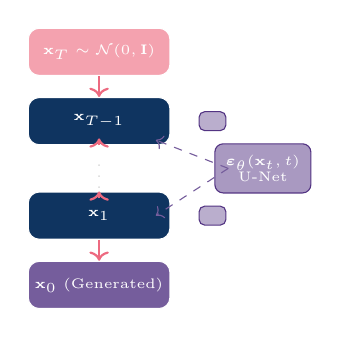
\begin{tikzpicture}[scale=0.80,
        box/.style={rounded corners=4pt,draw=white!40,
                    fill=AccentBlue,minimum width=1.8cm,
                    minimum height=0.6cm,font=\tiny,text=white,
                    inner sep=2pt,align=center}]

        % noisy → clean (vertical)
        \node[box,fill=NeonPink!50] (xT) at (0,0) {$\x_T\sim\mathcal{N}(0,\mathbf{I})$};
        \node[box] (xT1) at (0,-1.1) {$\x_{T-1}$};
        \node[font=\tiny,text=LightGray] (dots) at (0,-1.85) {$\vdots$};
        \node[box] (x1)  at (0,-2.6) {$\x_1$};
        \node[box,fill=AccentPurple!80] (x0)  at (0,-3.7) {$\x_0$ (Generated)};

        \foreach \a/\b in {xT/xT1,xT1/dots,dots/x1,x1/x0}{
          \draw[->,thick,NeonPink!80] (\a) -- (\b);
        }

        % network annotations
        \foreach \y in {-1.1,-2.6}{
          \node[draw=AccentPurple,rounded corners=2pt,
                fill=AccentPurple!40,font=\tiny,text=white,
          minimum width=0.34cm,minimum height=0.24cm,
          inner sep=0pt] at (1.8,\y)
                {};
        }
        \node[draw=AccentPurple,rounded corners=3pt,
              fill=AccentPurple!50,font=\tiny,text=white,
              inner sep=4pt,align=center] at (2.6,-1.85)
              {$\eps_\theta(\x_t,t)$\\U-Net};
        \draw[dashed,AccentPurple!80,->]
          (2.05,-1.85) -- (0.9,-1.4);
        \draw[dashed,AccentPurple!80,->]
          (2.05,-1.85) -- (0.9,-2.6);
      \end{tikzpicture}
  \end{columns}

\end{frame}

%══════════════════════════════════════════════════════════════════
\section{Training \& Score Matching}
%══════════════════════════════════════════════════════════════════

\begin{frame}{Training Objective}

  \begin{block}{Training Idea (Simple Version)}
    \vspace{-2pt}
    \begin{equation*}
      \mathcal{L}_{\text{simple}} =
        \mathbb{E}_{t,\,\x_0,\,\eps}\!\left[
          \left\|\,\eps \;-\;
          \eps_\theta\!\left(\sqrt{\bar\alpha_t}\,\x_0 +
          \sqrt{1-\bar\alpha_t}\,\eps,\; t\right)\right\|^2
        \right]
    \end{equation*}
  \end{block}

  \vspace{8pt}
  \begin{columns}[T]
    \column{0.48\textwidth}
      \textbf{Algorithm — Training}
      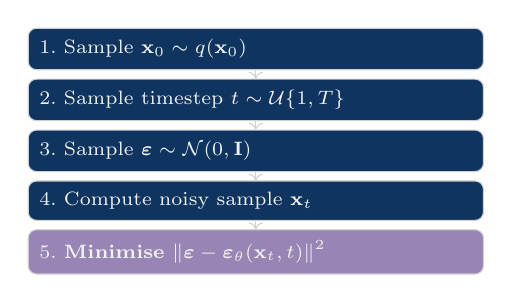
\begin{tikzpicture}[
        flowstep/.style={rounded corners=3pt,draw=LightGray,
                     fill=AccentBlue,text=SoftWhite,
                     text width=5.5cm,font=\scriptsize,
                     inner sep=4pt,align=left}]
        \node[flowstep] (s1) {1.~Sample $\x_0\sim q(\x_0)$};
        \node[flowstep,below=3pt of s1] (s2)
              {2.~Sample timestep $t\sim\mathcal{U}\{1,T\}$};
        \node[flowstep,below=3pt of s2] (s3)
              {3.~Sample $\eps\sim\mathcal{N}(0,\mathbf{I})$};
        \node[flowstep,below=3pt of s3] (s4)
              {4.~Compute noisy sample $\x_t$};
        \node[flowstep,below=3pt of s4,fill=AccentPurple!60] (s5)
              {5.~\textbf{Minimise} $\|\eps - \eps_\theta(\x_t,t)\|^2$};
        \foreach \a/\b in {s1/s2,s2/s3,s3/s4,s4/s5}{
          \draw[->,LightGray] (\a.south) -- (\b.north);
        }
      \end{tikzpicture}

    \column{0.48\textwidth}
      \textbf{What this loss means}\\[4pt]
      \small
      \begin{itemize}
        \item We add known noise to a clean sample
        \item The model guesses that exact noise
        \item If guess is close, the model is learning correctly
        \item After training, we can remove noise step by step
      \end{itemize}
      \vspace{4pt}
      \highlight{Key insight}: learning to denoise is enough for generation.
  \end{columns}

\end{frame}

%──────────────────────────────────────────────────────────────────
\begin{frame}{Noise Schedule \& Sampling Speed}
  \begin{columns}[T]
    \column{0.50\textwidth}
      \textbf{Noise Schedules}
      \begin{itemize}
        \item \textit{Linear}: increase noise at a constant rate
        \item \textit{Cosine}: keeps more structure early on
        \item \textit{Learned}: schedule is optimized by data
      \end{itemize}

      \vspace{6pt}
      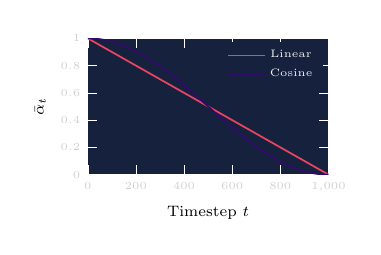
\begin{tikzpicture}[scale=0.78]
        \begin{axis}[
          width=5.5cm,height=3.8cm,
          xlabel={\scriptsize Timestep $t$},
          ylabel={\scriptsize $\bar\alpha_t$},
          axis background/.style={fill=MidBlue},
          axis line style={white},
          tick style={white},
          ticklabel style={font=\tiny,text=LightGray},
          legend style={font=\tiny,fill=MidBlue,
                        text=SoftWhite,draw=none},
          xmin=0,xmax=1000,ymin=0,ymax=1]
          \addplot[thick,NeonPink,domain=0:1000,samples=80]
            {(1000-x)/1000};
          \addlegendentry{Linear}
          \addplot[thick,AccentPurple!120,domain=0:1000,samples=80]
            {0.5*(1+cos(deg(3.14159*(x/1000))))};
          \addlegendentry{Cosine}
        \end{axis}
      \end{tikzpicture}

    \column{0.48\textwidth}
      \textbf{Accelerated Sampling}
      \begin{itemize}
        \item DDPM: $T=1000$ steps (slow)
        \item \highlight{DDIM} (Song et al., 2020): deterministic,
              $\sim$50 steps, same quality
        \item \highlight{DPM-Solver}: $\sim$20 steps
        \item \highlight{Consistency Models}: 1–2 steps!
      \end{itemize}

      \vspace{4pt}
      \small Speed-quality trade-off is an active research frontier.
  \end{columns}
\end{frame}

%══════════════════════════════════════════════════════════════════
\section{Applications}
%══════════════════════════════════════════════════════════════════

\begin{frame}{Applications \& Variants}
  \begin{columns}[T]
    \column{0.60\textwidth}
      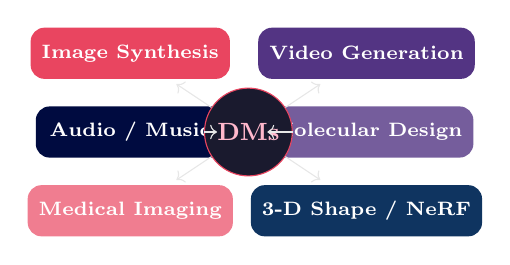
\begin{tikzpicture}[
        app/.style={rounded corners=5pt,
                    minimum width=2.4cm,minimum height=0.65cm,
                    font=\scriptsize\bfseries,text=white,
                    inner sep=4pt,align=center},
        every node/.style={font=\scriptsize}]

        \node[app,fill=NeonPink]      (img) at (0,0)     {Image Synthesis};
        \node[app,fill=AccentPurple]  (vid) at (3,0)     {Video Generation};
        \node[app,fill=AccentBlue!120](aud) at (0,-1.0)  {Audio / Music};
        \node[app,fill=AccentPurple!80](mol) at (3,-1.0) {Molecular Design};
        \node[app,fill=NeonPink!70]   (med) at (0,-2.0)  {Medical Imaging};
        \node[app,fill=AccentBlue]    (3d)  at (3,-2.0)  {3-D Shape / NeRF};

        \node[draw=NeonPink,circle,fill=DarkBlue,
            font=\small\bfseries,text=AccentText,
              minimum size=1.1cm] (c) at (1.5,-1.0) {DMs};

        \foreach \n in {img,vid,aud,mol,med,3d}{
          \draw[LightGray!50,->,shorten >=3pt] (c) -- (\n);
        }
      \end{tikzpicture}

    \column{0.38\textwidth}
      \textbf{Conditional Generation}
      \begin{itemize}
        \item \textbf{Classifier guidance}: steer outputs to a target label
        \item \textbf{Classifier-free}: steer generation without a separate classifier
        \item \textbf{Text conditioning}: prompt-based image generation
      \end{itemize}

      \vspace{4pt}
      \soft{\footnotesize Notable: Stable Diffusion (latent space),
      DALL·E 3 (GPT captions), Sora (video)}
  \end{columns}
\end{frame}

%══════════════════════════════════════════════════════════════════
\section{Conclusion}
%══════════════════════════════════════════════════════════════════

\begin{frame}{Takeaways \& Open Challenges}
  \begin{columns}[T]
    \column{0.50\textwidth}
      \begin{block}{\faIcon{check-circle}~Key Takeaways}
        \begin{itemize}
          \item Diffusion = iterative \textbf{denoising}
          \item Training objective is \textbf{simple MSE}
          \item Grounded in \textbf{score matching} theory
          \item Sets \textbf{state-of-the-art} across modalities
        \end{itemize}
      \end{block}

    \column{0.48\textwidth}
      \begin{block}{\faIcon{flask}~Open Challenges}
        \begin{itemize}
          \item Slow sampling (active research)
          \item High compute cost
          \item Evaluation metrics (FID, CLIP-S)
          \item Alignment \& safety of generated content
        \end{itemize}
      \end{block}
  \end{columns}

  \vspace{10pt}
  \begin{center}
    
\begin{tikzpicture}
      \node[draw=NeonPink,rounded corners=6pt,
            fill=AccentBlue!70,
            text=SoftWhite,inner sep=10pt,
            text width=11cm,align=center]{
        \textbf{Core Formula to Remember}\\[4pt]
        $\displaystyle
          \mathcal{L} =
          \mathbb{E}_{t,\x_0,\eps}\!\left[
            \bigl\|\eps - \eps_\theta\!\bigl(\sqrt{\bar\alpha_t}\,\x_0
            + \sqrt{1-\bar\alpha_t}\,\eps,\;t\bigr)\bigr\|^2
          \right]$
      };
    \end{tikzpicture}
  \end{center}
\end{frame}

%──────────────────────────────────────────────────────────────────
% THANK YOU SLIDE
%──────────────────────────────────────────────────────────────────
{
\setbeamercolor{background canvas}{bg=DarkBlue}
\begin{frame}[plain]
  \begin{tikzpicture}[remember picture,overlay]
    \foreach \r/\op in {6/0.04,4/0.07,2.2/0.11}{
      \fill[NeonPink,opacity=\op]
        (current page.center) circle (\r cm);
    }
  \end{tikzpicture}
  \vspace{2cm}
  \begin{center}
    {\Huge\bfseries\color{SoftWhite} Thank You!}\\[12pt]
    {\large\color{LightGray} Thanks for listening}\\[18pt]
    {\small\color{LightGray}
     Ho et al.\ (2020) — \textit{Denoising Diffusion Probabilistic Models}\\
     Song \& Ermon (2019) — \textit{Score-Based Generative Modelling}\\
     Song et al.\ (2020) — \textit{DDIM}\\
     Nichol \& Dhariwal (2021) — \textit{Improved DDPM}}
  \end{center}
\end{frame}
}

\end{document}